\chapter{Topological Stability as MNP}

\section{ General idea of the topological stability }

\subsection{Alternative with a persistent homology}


\subsection{ Transition to the spectral properties }





\section{ 101 on Spectral Matrix Nearness Problems }

\todo{definition}

Generally speaking, for a given matrix \( A \) a \emph{matrix nearness problem} consists of finding the closest possible matrix \( X \) among the admissible set with a number of desired properties. For instance, one may search for the closest (in some metric) symmetric positive/negative definite matrix, unitary matrix or the closest graph Laplacian. 

Motivated by the topological meaning of the \emph{kernel} of Hodge Laplacians \( L_k \), we assume the specific case of \emph{spectral} MNPs: here one aims for the target matrix \( X \) to have a specific spectrum \( \sigma(X) \). For instance in the stability study of the dynamical system \( \dot{\b x} = A \b x \) one can search for the closest Hurwitz matrix such that \( \mathrm{Re} \left[ \lambda_i \right] < 0 \) for all \( \lambda_i \in \sigma(X) \); similarly, assuming given matrix \( A \) is a graph Laplacian, one can search for the closest disconnected graph (so the algebraic connectivity \( \lambda_2 = 0 \)).

Here we recite the optimization framework developed by REFREFREF\todo{fix it} for the class of the spectral matrix nearness problems; one should note, however, that this is by far not the only approach to the task, REFREFREF\todo{also fix it with Nicholas and others, I guess?}.

\subsection{Functional and Gradient Flow}

Let as assume that \( X = A + \Delta \) and intead of searching for \( X \), we search for the perturbation matrix \( \Delta \); additionally, we assume that \( \Omega \) is the admissible set containing all possible perturbations \( \Delta \).


\subsection{ Transition to the gradient flow }
  
  \todo{ Derivative }

\subsection{ Constraint gradient flow }

\subsection{ Sparsity pattern and rank-1 optimizers }

\subsection{ Idea of two level optimization }















\section{Direct approach: failure and discontinuity problems }


\subsection{Principal spectral inheritance}


Before moving on to the next section, we recall here a relatively direct  but important spectral property that connects the spectra of the $k$-th and $(k+1)$-th order Laplacians. 

\begin{theorem}[HOL's spectral inheritance]\label{thm:inherit}
  Let $L_k$ and $L_{k+1}$ be  higher-order Laplacians for the same simplicial complex $\mc K$. Let $\bar L_k=\bar L_k^{down}+\bar L_k^{up}$, where $\bar L_k^{down}=\bar B_k^\top \bar B_k$ and $\bar L_k^{up}=\bar B_{k+1} \bar B_{k+1}^\top$. Then:
  \begin{enumerate}
    \item $\sigma_+(\bar L_k^{up})=\sigma_+(\bar L_{k+1}^{down})$, where $\sigma_+(\cdot)$ denotes the positive part of the spectrum;
    \item if $ 0 \ne \mu \in \sigma_+(\bar L_k^{up}) = \sigma_+(\bar L_{k+1}^{down})$, then the eigenvectors are related as follows:
    \begin{enumerate}
      \item if $\b x$ is and eigenvector for $\bar L_k^{up}$ with the eigenvalue $\mu$, then $\b y = \frac{1}{\sqrt{\mu}} \bar B_{k+1}^\top \b x$ is an eigenvector for $\bar L_{k+1}^{down}$ with the same eigenvalue;
      \item if $\b u$ is and eigenvector for $\bar L_{k+1}^{down}$ with the eigenvalue $\mu$ and $\b u \notin \ker \bar B_{k+1}$, then $\b v = \frac{1}{\sqrt{\mu}} \bar B_{k+1} \b u$ is an eigenvector for $\bar L_{k}^{up}$ with the same eigenvalue;
    \end{enumerate}
    \item for each Laplacian $\bar L_k$: if $\b v \notin \ker \bar L_k^{down}$ is the eigenvector for $\bar L_k^{down}$, then $\b v \in \ker \bar L_{k}^{up}$; vice versa, if $\b u \notin \ker \bar L_k^{up}$ is the eigenvector for $\bar L_k^{up}$, then $\b v \in \ker \bar L_k^{down}$;
    \item consequently, there exist $\mu \in \sigma_+(\bar L_k)$ with an eigenvector $\b u \in \ker \bar L_k^{up}$, and $\nu \in \sigma_+(\bar L_{k+1})$ with an eigenvector $\b u \in \ker \bar L_{k+1}^{down}$, such that:
    $$
    \bar B_k^\top \bar B_k \b v  = \mu \b v, \qquad \bar B_{k+2} \bar B_{k+2}^\top \b u = \nu \b u\, . 
    $$
  \end{enumerate}
\end{theorem}
\begin{proof}
For $(2a)$ it is sufficient to note that $ \bar L_{k+1}^{down} \b y = \bar B_{k+1}^\top \bar B_{k+1} \frac{1}{\sqrt{\mu}} \bar B_{k+1}^\top \b x = \frac{1}{\sqrt{\mu}}\bar B_{k+1}^\top \bar L_k^{up} \b x = \sqrt \mu \bar B_{k+1}^\top \b x  = \mu \b y$. Similarly, for $(2b)$: $\bar L_k^{up} \b v= \bar B_{k+1} \bar B_{k+1}^\top \frac{1}{\sqrt{\mu}} \bar B_{k+1} \b u = \frac{1}{\sqrt{\mu}} \bar B_{k+1} \bar L_{k+1}^{down} \b u = \mu \b v $; joint $2(a)$ and $2(b)$ yield $(1)$. \emph{Hodge decomposition} immediately yields the strict separation of eigenvectors between $\bar L_k^{up}$ and $\bar L_k^{down}$, $(3)$; given $(3)$, all the inherited  eigenvectors from $(2a)$ fall into the $\ker \bar L_{k+1}^{down}$, thus resulting into $(4)$.
\end{proof}
In other words, the variation of the spectrum of the $k$-th Laplacian when moving from one order to the next one works as follows: 
the down-term $\bar L_{k+1}^{down}$ inherits the positive part of the spectrum from the up-term of  $\bar L_k^{up}$; the  eigenvectors corresponding to the inherited positive part of the spectrum lie in the kernel of $\bar L_{k+1}^{up}$; at the same time, the ``new'' up-term $\bar L_{k+1}^{up}$ has a new, non-inherited, part of the positive spectrum (which, in turn, lies in the kernel of the $(k+2)$-th down-term).

In particular, we notice that for $k = 0$, since $B_0=0$ and $\bar L_0=\bar L_0^{up}$, the  theorem yields $\sigma_+ (\bar L_0 ) = \sigma_+ (\bar{L_1}^{down}) \subseteq \sigma_+(\bar L_1)$. In other terms, the positive spectrum of the $\bar L_0$ is inherited by the spectrum of $\bar L_1$ and the remaining (non-inherited) part of $\sigma_+(\bar L_1)$ coincides with $\sigma_+(\bar L_1^{up})$. 
\Cref{fig:thm_spct_ill} provides an  illustration of the statement of  \Cref{thm:inherit} for $k = 0$.
  \begin{figure}[t]
    \centering
    \begin{tikzpicture}
      \node[draw] at (0,0) {0};
      \node[draw] at (0.5,0) {0};
      \node at (1, 0) {$\cdots$};
      \node[draw] at (1.5,0) {0};
      \node[draw, fill=bananamania] at (2.15,0) {\tiny{$\lambda_1$}};
      \node[draw, fill=bananamania] at (2.65,0) {\tiny{$\lambda_2$}};
      \node[draw, fill=burntsienna] at (3.15,0) {\tiny{$\lambda_3$}};
      \node[draw, fill=bananamania] at (3.65,0) {\tiny{$\lambda_4$}};
      \node[draw, fill=burntsienna] at (4.15,0) {\tiny{$\lambda_5$}};
      \node[draw, fill=burntsienna] at (4.65,0) {\tiny{$\lambda_6$}};
      \node[draw, fill=bananamania] at (5.15,0) {\tiny{$\lambda_7$}};
      \node[draw, fill=bananamania] at (5.65,0) {\tiny{$\lambda_8$}};
      \node[draw, fill=burntsienna] at (6.15,0) {\tiny{$\lambda_9$}};
      \node[draw, fill=bananamania] at (6.65,0) {\tiny{$\lambda_{10}$}};
      \node at (8.5, 0) {$\leftarrow \quad \sigma (\bar L_1)$\phantom{$\bar B_1$}};
    
      \node[draw] at (0,-0.7) {0};
      \node[draw] at (0.5,-0.7) {0};
      \node at (1, -0.7) {$\cdots$};
      \node[draw] at (1.5,-0.7) {0};
      \node[draw, fill=bananamania] at (2.15,-0.7) {\tiny{$\lambda_1$}};
      \node[draw, fill=bananamania] at (2.65,-0.7) {\tiny{$\lambda_2$}};
      \node[draw] at (3.15,-0.7) {0};
      \node[draw, fill=bananamania] at (3.65,-0.7) {\tiny{$\lambda_4$}};
      \node[draw] at (4.15,-0.7) {0};
      \node[draw] at (4.65,-0.7) {0};
      \node[draw, fill=bananamania] at (5.15,-0.7) {\tiny{$\lambda_7$}};
      \node[draw, fill=bananamania] at (5.65,-0.7) {\tiny{$\lambda_8$}};
      \node[draw] at (6.15,-0.7) {0};
      \node[draw, fill=bananamania] at (6.65,-0.7) {\tiny{$\lambda_{10}$}};
      \node at (8.5, -0.7) {$\leftarrow \quad \sigma (\bar B_1^T \bar B_1)$};
    
      \node[draw] at (0,-1.4) {0};
      \node[draw] at (0.5,-1.4) {0};
      \node at (1, -1.4) {$\cdots$};
      \node[draw] at (1.5,-1.4) {0};
      \node[draw] at (2.15,-1.4) {0};
      \node[draw] at (2.65,-1.4) {0};
      \node[draw, fill=burntsienna] at (3.15,-1.4) {\tiny{$\lambda_3$}};
      \node[draw] at (3.65,-1.4) {0};
      \node[draw, fill=burntsienna] at (4.15,-1.4) {\tiny{$\lambda_5$}};
      \node[draw, fill=burntsienna] at (4.65,-1.4) {\tiny{$\lambda_6$}};
      \node[draw] at (5.15,-1.4) {0};
      \node[draw] at (5.65,-1.4) {0};
      \node[draw, fill=burntsienna] at (6.15,-1.4) {\tiny{$\lambda_9$}};
      \node[draw] at (6.65,-1.4) {0};
      \node at (8.5, -1.4) {$\leftarrow \quad \sigma (\bar B_2 \bar B_2^T)$};
    
      \draw [
        thick,
        decoration={
            brace,
            mirror,
            raise=0.25cm
        },
        decorate
      ] (-0.25, -1.4) -- (1.75, -1.4) 
    node [pos=0.5,anchor=north,yshift=-0.25cm] {holes}; 
      \draw[pattern=north west lines] (1.75,0.4) rectangle (1.85, -1.8);
      \node[draw, align=center, fill=bananamania] at (1.8,-2.1) {$\mu$};
    \end{tikzpicture}
    \caption{Illustration for the principal spectrum inheritance (\Cref{thm:inherit}) in case $k=0$: spectra of $\bar L_1$, $\bar {\Ld 1}$ and $\bar {\Ld 1}$ are shown. Colors signify the splitting of the spectrum, $\lambda_i>0 \in \sigma(\bar L_1)$ ; all yellow eigenvalues are inherited from $\sigma_+(\bar L_0)$; red eigenvalues belong to the non-inherited part. Dashed barrier $\mu$ signifies the penalization threshold (see the target functional in \Cref{subsec:functional}) preventing homological pollution (see \Cref{subsec:connetedness}). }
    \label{fig:thm_spct_ill}
    \vspace{-10pt}
  \end{figure}


\subsection{ Example with inheritted disconnectedness }



\subsection{ Example with faux edges (different weighting scheme) }





\section{ Functional, derivative and alternating scheme }

\subsection{ Target Functional }


\subsection{ Free gradient calculation }

\begin{theorem}[Derivative of simple eigenvalues]\label{lem:eigderiv} 
  Consider a continuously differentiable path of square symmetric matrices $A(t)$ for $t$ in an open interval $\mc I$. Let $\lambda(t)$, $t\in \mc I$, be a continuous path of simple eigenvalues of $A(t)$. Let $\vec x(t)$ be the eigenvector associated to the eigenvalue $\lambda(t)$ and assume
  $\| \vec x(t) \| = 1$ for all $t$. 
  Then $\lambda$ is continuously differentiable on $\mc I$ with the derivative (denoted by a dot) 
  \begin{equation}
  \dot{\lambda} = \vec x^\top \dot{A} \vec x = \langle \vec  x \vec x^\top, \dot A \rangle\,.
  \end{equation}
  Moreover, ``continuously differentiable'' can be replaced with ``analytic'' in the assumption and the conclusion.
  \end{theorem}
  
  Let us denote the perturbed weight matrix by $\tilde W_1 (t) = W_1 + \eps E(t)$, and the corresponding $\tilde W_0 (t) = W_0(\tilde W_1(t))$ and $ \tilde W_2 (t) = W_2 (\tilde W_1(t) )$, defined accordingly as discussed in Section~\ref{sec:nearest_complex}. From now on
  we omit the time dependence for the perturbed matrices to simplify the notation.  
  Since $\tilde W_0$, $\tilde W_1$ and $\tilde W_2$ are necessarily diagonal, by the chain rule we have $\dot{\tilde{W}}_i (t) = \eps \diag \left( J_1^i  \dot E \vec 1  \right)$, where $\vec 1$ is the vector of all ones, $\diag(\vec v)$ is the diagonal matrix with diagonal entries the vector $\vec v$, and  $J_1^i$ is the Jacobian matrix of the $i$-th weight matrix with respect to $\tilde W_1$, which for any $u_1\in \mathcal V_1$ and $u_2 \in \mathcal V_i$, has entries 
  \(
      [J_1^i]_{u_1,u_2}=\frac{\partial }{\partial \tilde{w}_1{(u_1)}}\tilde{w}_i{(u_2)}\, .
  \)
  
  Next, in the following two lemmas, we express the time derivative of the Laplacian $\bar L_0$ and $\bar L_1^{up}$ as functions of $E(t)$. The proofs of these results are  straightforward and omitted for brevity. In what follows, $\Sym[A]$ denotes the symmetric part of the matrix $A$, namely $\Sym[A] = (A+A^\top)/2$.
  
  
  \begin{lemma}[Derivative of $\bar L_0$]
    \label{lem:eigderL0} 
    For the simplicial complex $\mc K$ with the initial edges' weight matrix $W_1$ and  fixed perturbation norm $\eps$, let $E(t)$ be a smooth path and $\tilde W_0, \tilde W_1, \tilde W_2$ be corresponding perturbed weight matrices. Then,
    \begin{equation}
      \frac{1}{2\eps} \frac{d}{dt} \bar L_0 (t)  = \tilde W_0^{-1}  B_1 \tilde W_1 \dot E  B_1^\top \tilde W_0^{-1}-\Sym\left[ \tilde W_0^{-1} \diag \left(  J_1^0 \dot E \vec 1 \right)  \bar L_0 \right]. 
    \end{equation}
  \end{lemma}
  
  \begin{lemma}[Derivative of $\bar L_1^{up}$]
    \label{lem:eigderL1}
    For the simplicial complex $\mc K$ with the initial edges' weight matrix $W_1$ and fixed perturbation norm $\eps$,  let $E(t)$ be a smooth path and $\tilde W_0, \tilde W_1, \tilde W_2$ be corresponding perturbed weight matrices.  Then, 
    \begin{equation*}
     \frac{1}{2\eps} \frac{d}{dt} \bar L^{up}_1 (t)  =   - \Sym \left[ \tilde W_1^{-1} B_2 \tilde W_2^2 B_2^\top \tilde W_1^{-1} \dot E \tilde W_1^{-1} \right] 
   + \tilde W_1^{-1} B_2 \tilde W_2 \diag\left(  J_1^0 \dot E \vec 1  \right) B_2^\top \tilde W_1^{-1}
    \end{equation*}
  \end{lemma}
  
  Combining Lemma~\ref{lem:eigderiv} with  Lemma~\ref{lem:eigderL0} and Lemma~\ref{lem:eigderL1} we 
  obtain the following expression for the free gradient of the functional.
  \begin{theorem}[The free gradient of  $F(\eps, E)$]
    \label{thm:fk_grad}
    Assume the initial weight matrices $W_0$, $W_1$ and $W_2$,  as well as the parameters $\eps>0$, $\alpha>0$ and $\mu>0$, are given. 
    Additionally assume that $E(t)$ is a differentiable matrix-valued function such that the first non-zero eigenvalue $\lambda_+(\eps, E)$ of $\bar L_1^{up}(\eps, E)$ and the second smallest eigenvalue $\mu_2(\eps, E)$ of $\bar L_0(\eps, E)$  are simple.  Let $\tilde W_0, \tilde W_1, \tilde W_2$ be corresponding perturbed weight matrices; then: 
   \begin{equation*}
        \begin{aligned}
      \frac{1}{\eps} & \nabla_{E}  F(\eps, E)(t)   = \lambda_+(\eps,E) \bigcdot \\
      & \bigcdot \bigg[ \Sym \left[  - \tilde W_1^{-1} B_2 \tilde W_2^2 B_2^\top \tilde W_1^{-1} \vec x_+ \vec x_+^\top \tilde W_1^{-1}     \right]  \\  &+ \diag \left(  {J_1^2}^\top \vect \left( B_2^\top \tilde W_1^{-1} \vec x_+ \vec x_+^\top \tilde W_1^{-1} B_2 \tilde W_2   \right)   \right) \bigg] - \frac{\alpha}{\mu} \max \left\{ 0, 1- \frac{\mu_2(\eps, E)}{\mu }\right\}  \bigcdot \\
      & \bigcdot \bigg[  B_1^\top \tilde W_0^{-1} \vec y_2 \vec y_2^\top \tilde W_0^{-1} B_1 \tilde W_1    - \diag \left( {J_1^0}^\top  \vect \left( \Sym[ \tilde W_0^{-1} \vec y_2 \vec y_2^\top \bar L_0 ] \right) \right) \bigg]
    \end{aligned} 
   \end{equation*}
    where $\vec x_+$ is a unit eigenvector of $\bar L_1^{up}$ corresponding to $\lambda_+$,  $\vec y_2$ is a unit eigenvector of $\bar L_0$ corresponding to $\mu_2$, and the operator $\vect (X)$ returns the main diagonal of $X$ as a vector. 
  \end{theorem}
  \begin{proof}
  To derive the expression for the gradient $\nabla_E F$, we exploit the chain rule for the time derivative: $\dot \lambda = \langle \frac{d}{dt} A(E(t)), \vec x \vec x^\top  \rangle = \langle \nabla_E \lambda, \dot E \rangle$. Then it is sufficient to apply the cyclic perturbation for the scalar products of Lemma~\ref{lem:eigderL0} and Lemma~\ref{lem:eigderL1} with $\vec x_+ \vec x_+^\top$ and $\vec y_2 \vec y_2^\top$ respectively. The final transition requires the formula:
   \begin{equation*}
     \left\langle A, \diag(B E \vec 1) \right\rangle = \scal{\diag \left(   B^\top (\vect A) \right) ,\, E}.
   \end{equation*}
  \end{proof}
  \begin{remark}
    The derivation above assumes the simplicity of both $\mu_2(\eps,E)$ and $\lambda_+(\eps,E)$. This assumption is not restrictive as simplicity for these extremal eigenvalues is a generic property. 
    Indeed we observe simplicity in all our numerical tests.  
  \end{remark}
  
  \subsection{The constrained gradient system and its stationary points}
  \label{subsec:constrained}
  In this section we are deriving from the free gradient determined in  Theorem~\ref{thm:fk_grad} the constrained gradient of the considered functional, that is the projected gradient (with respect to the Frobenius inner product) onto the manifold $\Omega \cap \Pi_\eps$,
  which consists of perturbations $E$ of unit norm which preserve the structure of $W$.
  
  In order to obtain the constrained gradient system, we need to project the unconstrained gradient given by 
  Theorem~\ref{thm:fk_grad} onto the feasible set and also to normalize $E$ to preserve its unit norm. 
  Using the Karush-Kuhn-Tucker conditions on a time interval where the set of $0$-weight edges remain unchanged, the projection is done via the mapping $\mathbb{P}_{+} G( \eps, E )$, where
  \[
  \left[\mathbb{P}_+ X \right]_{ij}=\begin{cases} X_{ij}, \quad \left[ W_1 + \eps E \right]_{ij}>0 \\ 0, \;\;\quad \text{otherwise} \end{cases}.
  \]
  Further, in order to comply with the constraint ${\| E(t) \|^2 =1}$, we must have 
  \begin{equation} \label{eq:normconstr}
   0 = \frac12\,\frac d{dt}\| E(t) \|^2= \langle E(t), \dot E(t) \rangle.
  \end{equation}
  Thus, we obtain the following constrained optimization problem for the admissible direction of the steepest descent
  
  \begin{lemma}[Direction of steepest admissible descent]
  \label{lem:opt} 
  Let $E,G\in{\mathbb R}^{m \times m}$ with $G$ given by (\ref{eq:traj_transition}), and 
  ${\|E\|=1}$. On a time interval where the set of $0$-weight edges remains unchanged, 
  the gradient system  reads
  \begin{equation}
    \label{eq:traj_proj}
    \dot{E}(t)=-\mathbb{P}_+ G( \eps, E(t) )+ \kappa  \mathbb{P}_+E(t), \quad \text{where} \quad 
    \kappa = \frac{\scal{ \eps, G(E(t) ),\, \mathbb{P}_+E(t)}}{  \lVert\mathbb{P}_+E(t)\rVert^2}.
   \end{equation}
  \end{lemma}
  \begin{proof}
  We need to orthogonalize $\dot{E}(t)$ with respect to $E(t)$. To this end, we introduce a linear orthogonality correction, i.e.\ we set  
  $\dot E = \mathbb{P}_+ (-G - \kappa E)$, 
  {and we determine} $\kappa$ {by imposing the} constraint $\langle E,\dot E \rangle =0$. We then have
  \[
  0=\langle E,\dot E \rangle = \langle E,\mathbb{P}_+ (-G - \kappa E) \rangle=
  - \langle \mathbb{P}_+  E,G \rangle -  \kappa\langle \mathbb{P}_+  E,\mathbb{P}_+  E \rangle,
  \]
  and the result follows.
  \end{proof}	
    
  Equation~(\ref{eq:traj_proj}) suggests that the system goes ``primarily'' in the direction of the antigradient $-G(\eps,E)$, thus the functional is expected to decrease along it.
  \begin{lemma}[Monotonicity]
  Let $E(t)$ of unit Frobenius norm satisfy the differential equation (\ref{eq:traj_proj}), with $G$ given by (\ref{eq:traj_transition}). Then, 
  $F(\eps, E(t))$ decreases monotonically with~$t$.
  \end{lemma}
  \begin{proof}
  We consider first the simpler case where the non-negativity projection does not apply so that $G=G(\eps,E)$ (without $\mathbb{P}_+$). Then
  \begin{equation}\label{eq:mono}
      \begin{aligned} 
    \frac{d}{dt} F(\eps, E)(t) & =\scal{  \nabla_{E} F_k(\eps, E), \, \dot{E} }=\scal{ \eps G( \eps, E(t) ) ,\, -G( \eps, E(t) )+\kappa E(t) } \\ 
    & = -\eps \lVert G( \eps, E ) \rVert^2 + \eps\frac{\scal{G( \eps, E ),\, E }}{\scal{E, \, E}} \scal{G( \eps, E ),\, E }  \\
    & = \eps \left(  -\lVert G( \eps, E ) \rVert^2 + \frac{\left| \scal{G( \eps, E ),\, E } \right|^2}{\lVert E \rVert^2} \right) \le 0 
  \end{aligned}
  \end{equation}
  where the final estimate is given by the Cauchy-Bunyakovsky-Schwarz inequality. The derived inequality holds on the time interval without the change in the support of $\mathbb P_+$ (so that no new edges are prohibited by the non-negativity projection).
  \end{proof}
  

\subsection{ Constrained gradient }


\subsection{ Alternating scheme }


\subsection{ Implementation }

\subsubsection{ Algorithms }

\subsubsection{ Computation of the first non-zero eigenvalue }

\subsubsection{ Preconditioning in the eigen-phase }







\section{ Benchmarking }

\subsection{Illustrative Example}\label{sec:illustrarive_example}

We consider here a small example 
of a simplicial complex $\mc K$ of order 2 
consisting of eight 0-simplices (vertices), twelve 1-simplices (edges),  four 2-simplices $\mc V_2 = \{[1,2,3], [1,2,8], [4,5,6],[5,6,7]\}$   and one corresponding hole $[2,3,4,5]$, hence, $\beta_1 = 1$. By design, the dimensionality of the homology group $\bar{\mc H}_1$ can be increased only by eliminating edges $[1,2]$ or $[5,6]$; for the chosen weight profile  $w_1([1,2]) > w_1([5,6])$, hence, the method should converge to the minimal perturbation norm $\eps = w_1([5,6])$ by eliminating the edge $[5,6]$, Figure~\ref{fig:illustrative_start}.


\begin{figure}[t]
    \centering
    \scalebox{0.7}{\begin{tikzpicture}
      \fill [opacity=0.25,liberty]    (0, 0) -- (2, 0) --  (1, 2) -- cycle;
       \fill [opacity=0.3,liberty]    (0, 0) -- (2, 0) --  (1, -2) -- cycle;
      \fill [opacity=0.5,liberty]    (4, 1) -- (3, 2.5) --  (5, 2.5) -- cycle;
      \fill [opacity=0.65,liberty]    (3, 2.5) -- (5, 2.5) --  (4, 4) -- cycle;
      \Vertex[x=0, y=0, style={color=liberty}, fontcolor=white, size=0.4, label = 6 ]{v1}
      \Vertex[x=2,y=0, style={color=liberty}, fontcolor=white, size=0.4, label = 5 ]{v2}
      \Vertex[x=1, y=2, style={color=liberty}, fontcolor=white, size=0.4, label=4]{v3}
      \Vertex[x=4, y=1, style={color=liberty}, fontcolor=white, size=0.4, label=3]{v4}
      \Vertex[x=3, y=2.5, style={color=liberty}, fontcolor=white, size=0.4, label=2]{v5}
      \Vertex[x=5, y=2.5, style={color=liberty}, fontcolor=white, size=0.4, label=1]{v6}
      \Vertex[x=4, y=4, style={color=liberty}, fontcolor=white, size=0.4, label=8]{v7}
      \Vertex[x=1, y=-2, style={liberty}, fontcolor=white, size = 0.4, label = 7]{v8}
      \Edge[Math, label=1](v1)(v2)
      \Edge[Math, label=0.6, lw=0.6pt](v1)(v3)
      \Edge[Math, label=2.2, lw=2.2pt](v2)(v3)
      \Edge[Math, label=0.7, lw=0.7](v2)(v4)
      \Edge[Math, label=2.5, lw=2.5](v3)(v5)
      \Edge[Math, label=1.8, lw=1.8](v4)(v5)
      \Edge[Math, label=1](v4)(v6)
      \Edge[Math, label=1.5, lw=1.5](v5)(v6)
      \Edge[Math, label=1.75, lw=1.75](v5)(v7)
      \Edge[Math, label=2, lw=2](v6)(v7)
      \Edge[Math, label=0.5,  lw =0.5pt](v1)(v8)
       \Edge[Math, label=3.0,  lw=3.0pt](v2)(v8)
  \end{tikzpicture}}
  \scalebox{0.7}{\begin{tikzpicture}
       \node at (-1, 0.5) {\large $\longrightarrow$};
      \fill [opacity=0.5,liberty]    (4, 1) -- (3, 2.5) --  (5, 2.5) -- cycle;
      \fill [opacity=0.65,liberty]    (3, 2.5) -- (5, 2.5) --  (4, 4) -- cycle;
      \Vertex[x=0, y=0, style={color=liberty}, fontcolor=white, size=0.4, label = 6 ]{v1}
      \Vertex[x=2,y=0, style={color=liberty}, fontcolor=white, size=0.4, label = 5 ]{v2}
      \Vertex[x=1, y=2, style={color=liberty}, fontcolor=white, size=0.4, label=4]{v3}
      \Vertex[x=4, y=1, style={color=liberty}, fontcolor=white, size=0.4, label=3]{v4}
      \Vertex[x=3, y=2.5, style={color=liberty}, fontcolor=white, size=0.4, label=2]{v5}
      \Vertex[x=5, y=2.5, style={color=liberty}, fontcolor=white, size=0.4, label=1]{v6}
      \Vertex[x=4, y=4, style={color=liberty}, fontcolor=white, size=0.4, label=8]{v7}
      \Vertex[x=1, y=-2, style={liberty}, fontcolor=white, size = 0.4, label = 7]{v8}
      %\Edge[Math, label=1](v1)(v2)
      \Edge[Math, label=0.6, lw=0.6pt](v1)(v3)
      \Edge[Math, label=2.2, lw=2.2pt](v2)(v3)
      \Edge[Math, label=0.7, lw=0.7](v2)(v4)
      \Edge[Math, label=2.5, lw=2.5](v3)(v5)
      \Edge[Math, label=1.8, lw=1.8](v4)(v5)
      \Edge[Math, label=1](v4)(v6)
      \Edge[Math, label=1.5, lw=1.5](v5)(v6)
      \Edge[Math, label=1.75, lw=1.75](v5)(v7)
      \Edge[Math, label=2, lw=2](v6)(v7)
      \Edge[Math, label=0.5,  lw =0.5pt](v1)(v8)
       \Edge[Math, label=3.0,  lw=3.0pt](v2)(v8)
  \end{tikzpicture}}
    \caption{
   % \brev
    Simplicial complex $\mc K$ on $8$ vertices for the illustrative run (on the left): all 2-simplices from $\mc V_2$ are shown in blue, the weight of each edge $w_1(e_i)$ is given on the figure. On the right: perturbed simplicial complex $\mc K$ through the elimination of the edge $[5,6]$ creating additional hole $[5, 6, 7, 8]$.
    \label{fig:illustrative_start}
    %\erev
    }
\end{figure}


\begin{figure}[t]
    \centering
    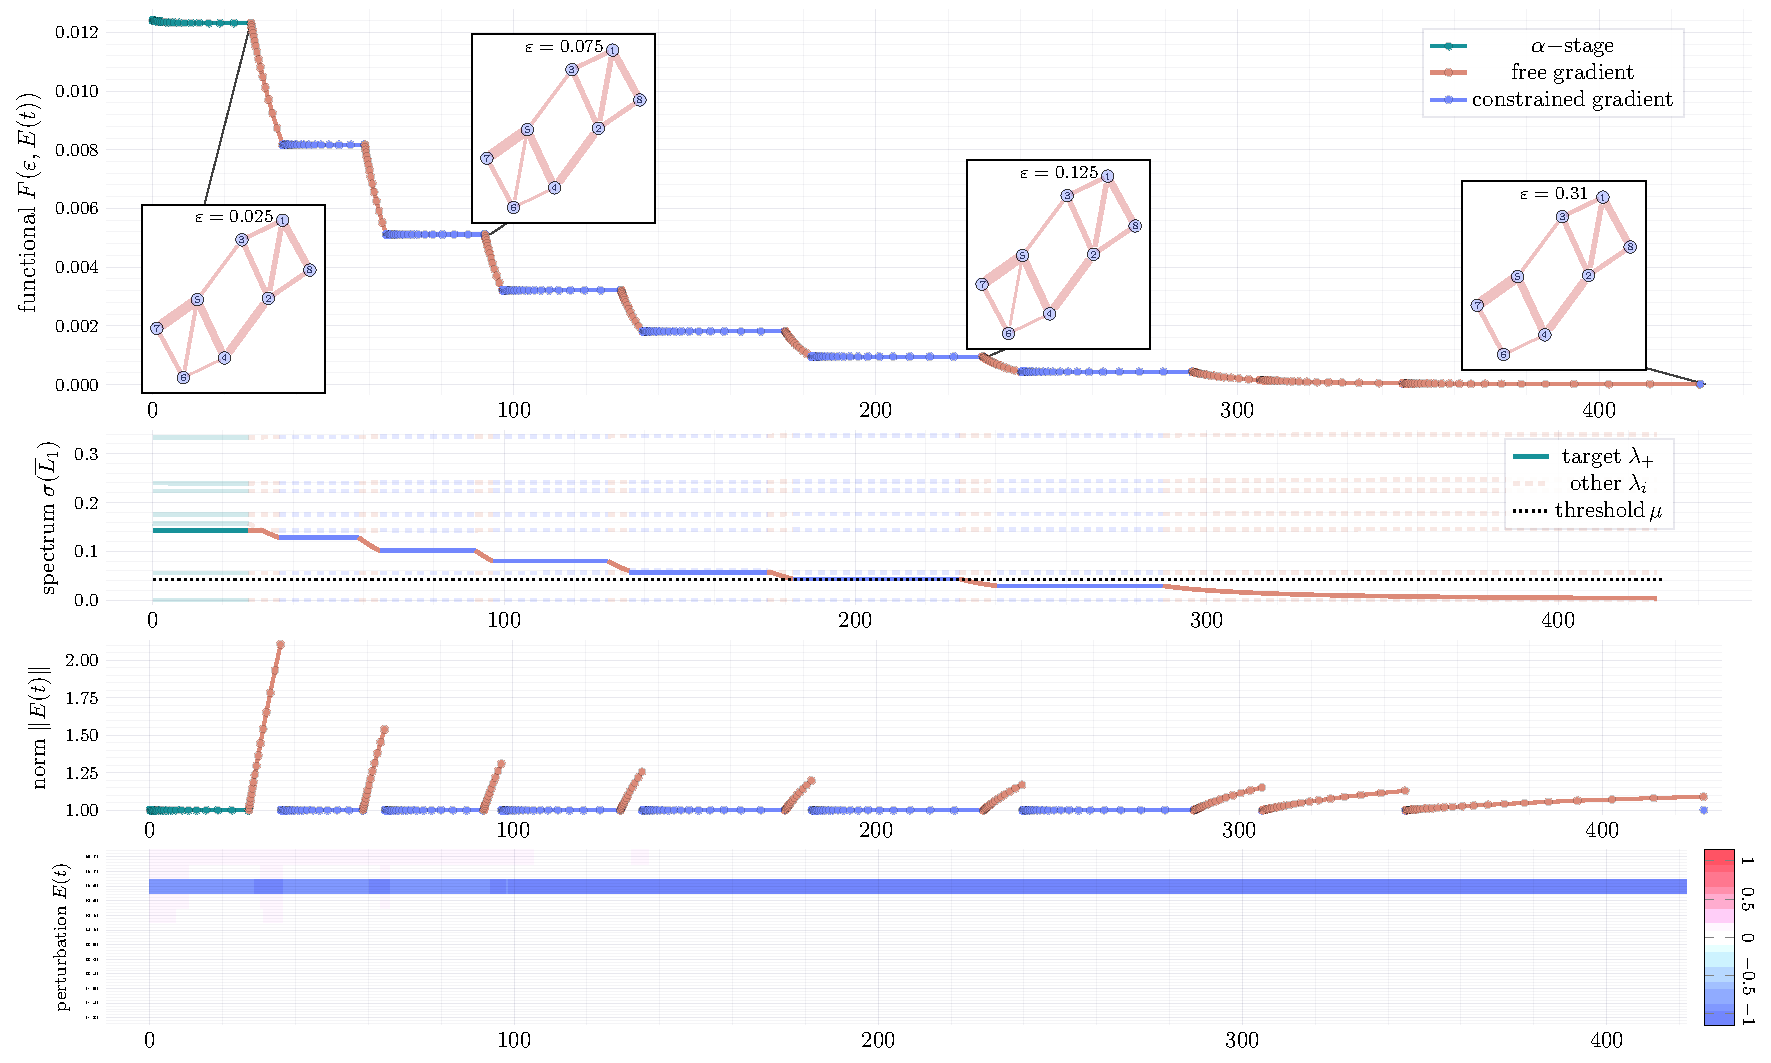
\includegraphics[width=1.0\textwidth,clip,trim=8pt 7pt 8pt 5pt]{figures/julia/test2.pdf}
    
    \caption{Illustrative run of the framework determining the topological stability: the top pane --- the flow of the functional $F(\eps, E(t))$; the second pane --- the flow of $\sigma(\bar L_1)$, $\lambda_+$ is highlighted; third pane --- the change of the perturbation norm $\| E(t) \|$; the bottom pane --- the heatmap of the perturbation profile $E(t)$.
     \label{fig:illustrative}
    }
\end{figure}

The exemplary run of the optimization framework in time is shown on Figure~\ref{fig:illustrative}.
The top panel of Figure~\ref{fig:illustrative} provides the continued flow of the target functional $F(\eps, E(t))$ consisting of the initial $\alpha$-phase (in green) and alternated constrained (in blue) and free gradient (in orange) stages. As stated above, $F(\eps, E(t))$ is strictly monotonic along the flow since the support of $\mathbb P_+$  does not change. Since the initial setup is not pathological with respect to the connectivity, the initial  $\alpha$-phase essentially reduces to a single constrained gradient flow and terminates after one run with $\alpha=\alpha_*$.  The constrained gradient stages are characterized by a slow changing $E(t)$, which is essentially due to the flow performing small adjustments to find the correct rotation on the unit sphere, whereas the free gradient stage quickly decreases the target functional.

The second panel shows the  behaviour of first non-zero eigenvalue $\lambda_+(\eps, E(t))$ (solid line) of $\bar L_1^{up}(\eps, E(t))$ dropping through the ranks of $\sigma(\bar L_1(\eps, E(t)))$ (semi-transparent); similar to the case of the target functional $F(\eps, E(t))$, $\lambda_+(\eps, E(t))$ monotonically decreases. The rest of the eigenvalues exhibit only minor changes, and the rapidly changing $\lambda_+$ successfully passes through the connectivity threshold $\mu$ (dotted line). 

The third and the fourth panels show the evolution of the norm of the perturbation $\| E(t) \|$ and the perturbation $E(t)$ itself, respectively.  The norm $\| E(t) \| $ is conserved during the constrained-gradient and the $\alpha$- stages; these stages correspond to the optimization of the perturbation shape, as shown by the small positive values at the beginning of the bottom panel which eventually vanish. During the free gradient integration the norm $\| E(t) \|$ increases, but the relative change of the norm declines with the growth of $\eps_i$ to avoid jumping over the smallest possible $\eps$. Finally, due to the simplicity of the complex, the  edge we want to eliminate, $56$, dominates the flow from the very beginning (see bottom panel); such a clear pattern persists only in small examples, whereas for large networks the perturbation profile is initially spread out among all the edges.


\subsection{Triangulation Benchmark}

To provide more insight into the computational behavior of the method, we synthesize here an almost planar 
graph dataset. Namely, we assume $N$ uniformly sampled vertices on the unit square with a network built by the Delaunay triangulation;  then, edges are randomly added or erased to obtain the sparsity $\nu$  (so that the graph has $\frac 12  \nu N(N-1)$ edges overall). An order-2 simplicial complex $\mc K=(\mc V_0,\mc V_1,\mc V_2)$  is then formed by letting $\mc V_0$ be the generated vertices, $\mc V_1$ the edges, and $\mc V_2$ every $3$-clique of the graph; edges' weights are sampled uniformly between $1/4$ and $3/4$, namely $w_1(e_i) \sim U [\frac{1}{4}, \frac{3}{4} ]$.


An  example of such triangulation is shown in Figure~\ref{fig:triang}; here $N=8$ and edges $[6, 8]$ and $[2, 7]$ were eliminated to achieve the desired sparsity.

\begin{figure}[t]
    \centering
    \subfloat[Example of Triangulation and Holes]{ \label{fig:triang}
        \scalebox{0.35}{\begin{tikzpicture}
      \Vertex[x=0, y=0, label=1, style={color=liberty}, fontcolor=white,]{v1}
      \Vertex[x=5, y=0, label=2, style={color=liberty}, fontcolor=white,]{v2}
      \Vertex[x=5, y=5, label=3, style={color=liberty}, fontcolor=white,]{v3}
      \Vertex[x=0, y=5, label=4, style={color=liberty}, fontcolor=white,]{v4}
      \Vertex[x=2, y=1.5, label=5, style={color=liberty}, fontcolor=white,]{v5}
      \Vertex[x=1, y=4, label=6, style={color=liberty}, fontcolor=white,]{v6}
      \Vertex[x=4, y=2.5, label=7, style={color=liberty}, fontcolor=white,]{v7}
      \Vertex[x=3, y=3.5, label=8, style={color=liberty}, fontcolor=white,]{v8}
      \Edge(v1)(v2)
      \Edge(v2)(v3)
      \Edge(v3)(v4)
      \Edge(v1)(v4)
      \Edge(v1)(v5)
      \Edge(v2)(v5)
      %\Edge(v2)(v7)
      \Edge(v3)(v7)
      \Edge(v5)(v7)
      \Edge(v7)(v8)
      \Edge(v5)(v8)
      \Edge(v5)(v6)
      %\Edge(v6)(v8)
      \Edge(v3)(v8)
      \Edge(v4)(v6)
      \Edge(v1)(v6)
      \Edge(v3)(v6)

      \fill [opacity=0.3,liberty]   (v1.center) -- (v2.center) -- (v5.center) -- cycle;
      \fill [opacity=0.3,liberty]   (v1.center) -- (v4.center) -- (v6.center) -- cycle;
      \fill [opacity=0.3,liberty]   (v1.center) -- (v5.center) -- (v6.center) -- cycle;
      \fill [opacity=0.3,liberty]   (v3.center) -- (v4.center) -- (v6.center) -- cycle;
      \fill [opacity=0.3,liberty]   (v5.center) -- (v7.center) -- (v8.center) -- cycle;
      \fill [opacity=0.3,liberty]   (v3.center) -- (v7.center) -- (v8.center) -- cycle;
      
      \Vertex[x=0, y=-3.5, style={color=white}]{fake}
  \end{tikzpicture}}
    }
    \subfloat[Time (in seconds)]{\label{fig:triang_time}
       \scalebox{0.33}{%\input{times_prec2.tex}
        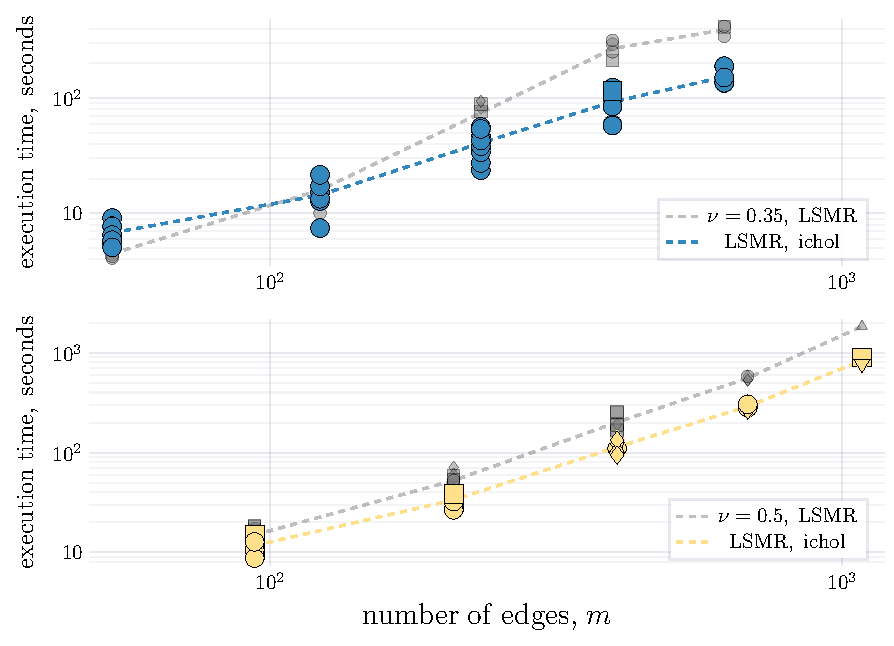
\includegraphics{figures/julia/times_prec2.pdf}
       }}
    \subfloat[Perturbation norm, $\eps$]{\label{fig:triang_eps}
        \scalebox{0.33}{%\input{eps_prec2.tex}
        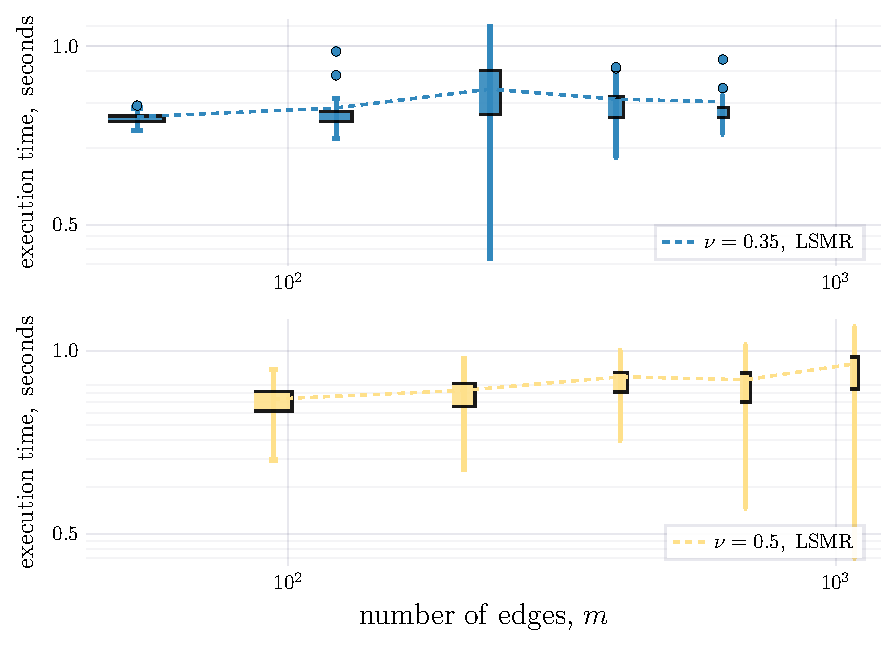
\includegraphics{figures/julia/eps_prec2.pdf}
        }}
        \caption{Benchmarking Results on the Synthetic Triangulation Dataset: varying sparsities $\nu=0.35, \, 0.5$ and $N=16, \, 22, \, 28, \, 34, \, 40$; each network is sampled $10$ times. Shapes correspond to the number of eliminated edges in the final perturbation: $1: \, \ocircle$, $2: \, \square$, $3: \pentagon$, $4: \, \triangle$. For each pair $(\nu, N)$, the un-preconditioned and Cholesky-preconditioned execution times are shown.}
        \vspace{-10pt}
\end{figure}

We sample networks with a varying number of vertices $N=10, \, 16, \, 22, \, 28$ and varying sparsity pattern $\nu=0.35, \, 0.5$ which determine the number of edges in the output  as $m = \nu \frac{N(N-1)}{2}$. Due to the highly randomized procedure, topological structures of a sampled graph with a fixed pair of parameters may differ substantially, so $10$ networks with the same $(N, \nu)$ pair are generated. For each network, the working time  (without considering the sampling itself) and the resulted perturbation norm $\eps$, and are reported in  Figure~\ref{fig:triang_time} and Figure~\ref{fig:triang_eps}, respectively. As anticipated in  Section~\ref{sec:computational_cost}, we show the performance of two implementations of the method, one based on LSMR and one based on LSMR preconditioned by using  the  incomplete Cholesky factorization of the initial matrices. We observe that, 
\begin{itemize}
    \item  the computational cost of the whole procedure  lies between $\mathcal O(m^2)$ and $\mathcal O(m^3)$ 
    \item denser structures, with a higher number of vertices, result in the higher number of edges being eliminated; at the same time, even most dense cases still can exhibit structures requiring the elimination of a single edge, showing that  the flow does not necessarily favor multi-edge optima;
    \item the required perturbation norm $\eps$ is growing with the size of the graph, Figure~\ref{fig:triang_eps}, but not too fast: it is expected that denser networks would require larger $\eps$ to create a new hole; at the same time if the perturbation were to grow drastically with the sparsity $\nu$, it would imply that the method tries to eliminate sufficiently more edges, a behavior that resembles convergence to a sub-optimal perturbation;
    \item preconditioning with a constant incomplete Cholesky multiplier, computed for the initial Laplacians, 
    provides a visible execution time gain for medium and large networks. Since the quality of the preconditioning deteriorates as the flow approaches the minimizer (as a non-zero eigenvalue becomes $0$), it is worth investigating the design of a preconditioner for the up-Laplacian that can be efficiently updated.
\end{itemize}


\subsection{Transportation Networks}

Finally, we provide an application to  real-world examples based on city transportation networks. 
We consider networks for Bologna, Anaheim, Berlin Mitte, and Berlin Tiergarten; each network consists of nodes --- intersections/public transport stops --- connected by edges (roads) and subdivided into zones; for each road the free flow time, length, speed limit are known; moreover, the travel demand for each pair of nodes is provided through the dataset of recorded trips.
All the datasets used here are publicly available at \url{https://github.com/bstabler/TransportationNetworks}; Bologna network is  provided by the Physic Department of the University of Bologna (enriched through the Google Maps API \url{https://developers.google.com/maps}).

The regularity of city maps naturally lacks $3$-cliques, hence forming the simplicial complex based on triangulations as done before frequently leads to trivial outcomes. 
Instead, here we ``lift'' the network to city zones, thus more effectively grouping the nodes in the graph. Specifically:
\begin{enumerate}
    \item we consider the completely connected graph where the nodes are zones in the city/region;
    \item the free flow time between two zones is temporarily assigned  as a weight of each edge: the time is as the shortest path between the zones (by the classic Dijkstra algorithm) 
    on the initial graph;
    \item similarly to what is done in the filtration used for persistent homology,  we filter out excessively distant nodes; additionally, we exclude the longest edges in each triangle in case it is equal to the sum of two other edges (so the triangle is degenerate and the trip by the longest edge is always performed through to others); 
    \item finally, we use the travel demand as an actual weight of the edges in the final network; travel demands are scaled \emph{logarithmically} via the transformation $w_i \mapsto \log_{10} \left(  \frac{w_i}{0.95 \min w_i} \right)$; see the example on the left panel of Figure~\ref{fig:bologna}.
\end{enumerate}
Given the definition of weights in the network, high instability (corresponding to small perturbation norm $\eps$) implies structural phenomena around the ``almost-hole'', where the faster and shorter route is sufficiently less demanded. 

\begin{figure}
    \centering
    \scalebox{1.0}[0.9]{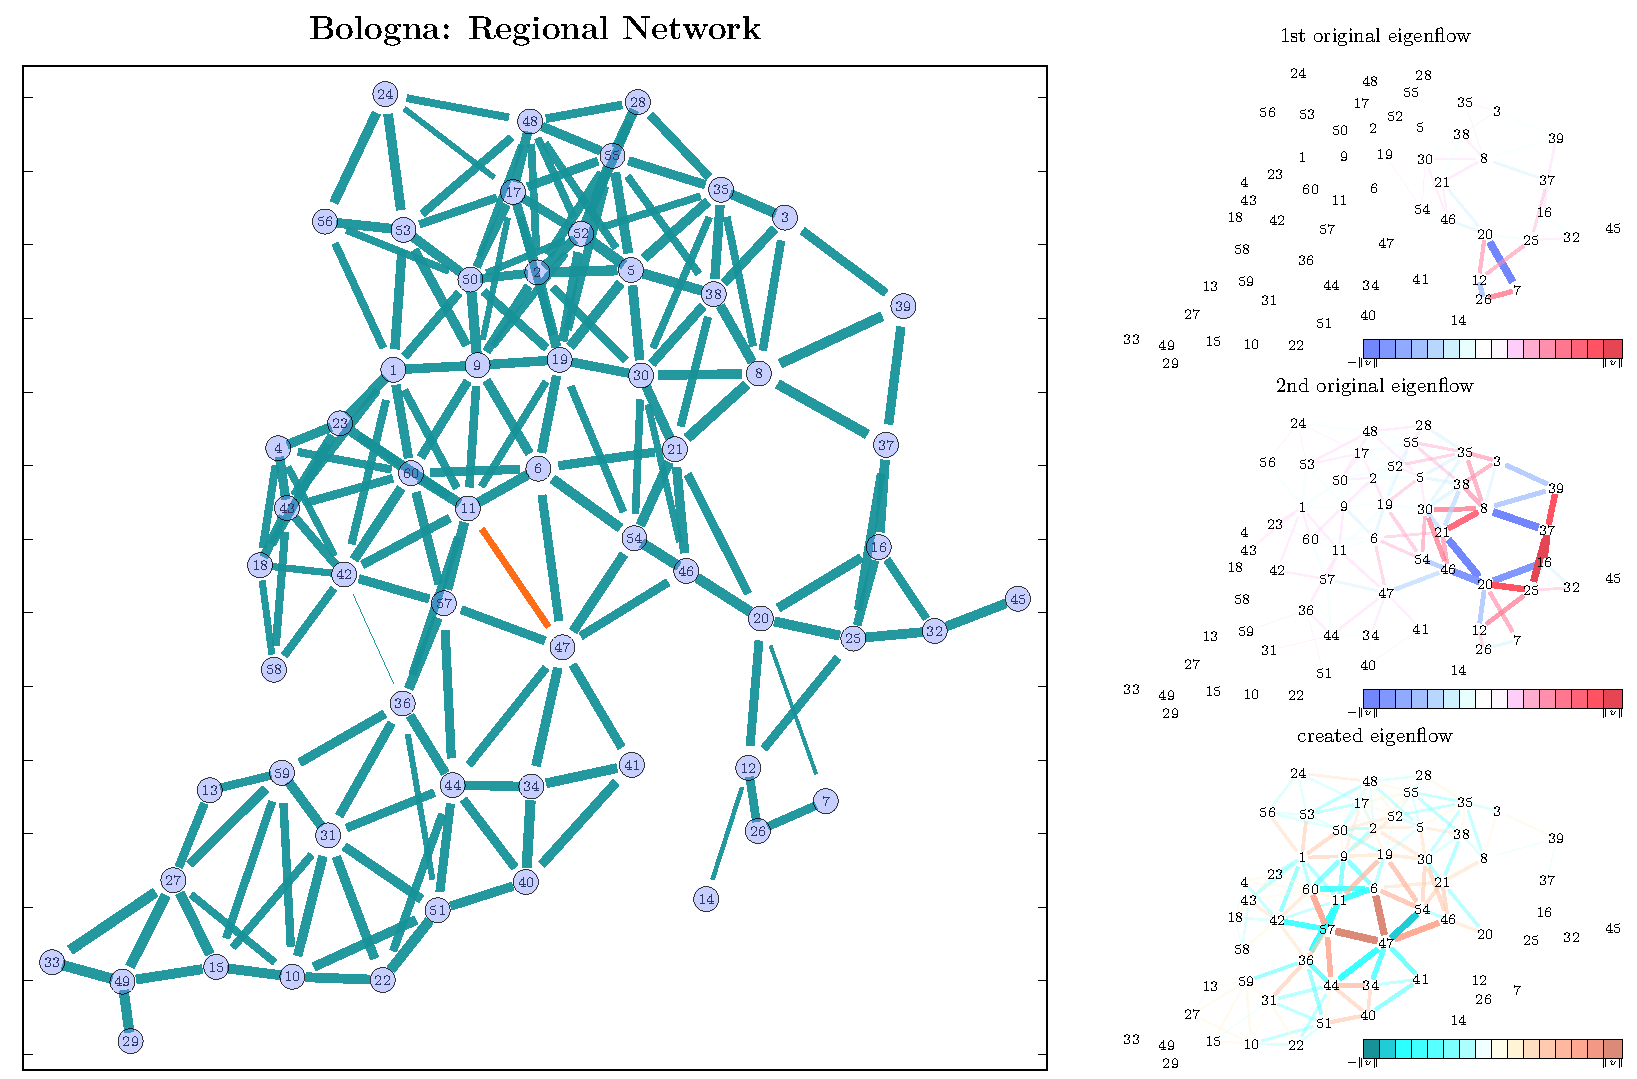
\includegraphics[width=1.0\columnwidth]{figures/julia/bologna.pdf}}
    \caption{Example of the Transportation Network for Bologna. Left pane: original zone graph where the width of edges corresponds to the weight, to-be-eliminated edge is colored in red. Right pane: eigenflows, original and created; color and width correspond to the magnitude of entries.}
    \label{fig:bologna}
\end{figure}


\begin{table}[hbtp]
  \centering
  \begin{NiceTabular}{@{}c!{\qquad}cccc!{\qquad}ccc@{}}
    \toprule
    \Block{2-1}{\bfseries Cities} & \Block{1-3}{\bfseries network} & & & \Block{2-1}{ \( \beta_1 \) } & \Block{1-3}{\bfseries logarithmic weights} \\
    & \( m_0 \) & \( m_1 \) & \( m_2 \) & & time & \( \eps \) & \( p \) \\
    \midrule
    \Block{2-1}{Bologna} & \Block{2-1}{60} & \Block{2-1}{175} & \Block{2-1}{171} & \Block{2-1}{2} &  \( 2.43 \)s & \( 0.65 \) & \( 0.003 \)\\
     &  &  &  & & \Block{1-3}{\small  \textbf{{[}11, 47{]}} ($4^{th}$ smallest) } \\[0.1cm]
     \dashedline
     \noalign{\vskip 0.1cm}
     \Block{2-1}{Anaheim} & \Block{2-1}{38} & \Block{2-1}{159} & \Block{2-1}{221} & \Block{2-1}{1} &  \( 5.39 \)s & \( 0.57 \) & \(0.003\)\\
     &  &  &  &  & \Block{1-3}{\small \textbf{{[}10, 29{]}} ($11^{th}$ smallest)} \\[0.1cm]
     \dashedline
     \noalign{\vskip 0.1cm}
     \Block{2-1}{Berlin-Tiergarten} & \Block{2-1}{26} & \Block{2-1}{63} & \Block{2-1}{55} & \Block{2-1}{0} & \(2.46\)s & \(1.18\) & \(0.015\) \\
     & &  & & & \Block{1-3}{\small \textbf{{[}6, 16{]}} ($20^{th}$ smallest)} \\[0.1cm]
     \dashedline
     \noalign{\vskip 0.1cm}
     \Block{2-1}{Berlin-Mitte} & \Block{2-1}{98} & \Block{2-1}{456} & \Block{2-1}{900} & \Block{2-1}{1} &  \( 127 \)s & \(0.887\) & \(0.0016\)\\
     & & & & & \Block{1-3}{\small \textbf{{[}57, 87{]}} ($6^{th}$), \textbf{{[}58, 87{]}}, ($17^{th}$) } \\
    \bottomrule
    \end{NiceTabular}

    \caption{
      Topological instability of the transportation networks: filtered zone networks with the corresponding perturbation norm \( \eps \) and its percentile among \( w_1(\cdot) \) profile. For each simplicial complex the number of nodes, edges and triangles in \( \mc V_2(\mc K) \) are provided alongside the initial number of holes \( \beta_1 \). The results of the algorithm consist of the perturbation norm, \( \eps \), computation time, and approximate percentile \( p \).\label{tab:bologna}
    }
  
\end{table}

In the case of Bologna, Figure~\ref{fig:bologna}, the algorithm eliminates the edge $[11, 47]$ (Casalecchio di Reno -- Pianoro) creating a new hole $6 - 11 - 57 - 47$. We also provide examples of the eigenflows in the kernel of the Hodge Laplacian (original and additional perturbed): original eigenvectors correspond to the circulations around holes $7-26-12-20$ and $8-21-20-16-37$ non-locally spread in the neighborhood~\cite{schaub2020random}. 

The results for four different networks are summarized in the Table~\ref{tab:bologna}; $p$ mimics the percentile, $\eps/\sum_{e\in \mc V_1}{w_i(e)}$, showing the overall small perturbation norm contextually. 
At the same time, we emphasize that except Bologna (which is influenced by the geographical topology of the land), the algorithm does not choose the smallest weight possible; indeed, given our interpretation of the topological instability, the complex for Berlin-Tiergarten is stable and the transportation network is effectively constructed.
































